\documentclass[10pt,journal,compsoc]{IEEEtran}

\usepackage[utf8]{inputenc}
\usepackage[T1]{fontenc}
\usepackage{cite}
\usepackage{amsmath,amssymb,amsfonts}
\usepackage{algorithmic}
\usepackage{graphicx}
\usepackage{textcomp}
\usepackage{xcolor}
\usepackage{booktabs}
\usepackage{pgfplots}
\usepackage{pgfplotstable}
\pgfplotsset{compat=1.18}
\usepackage{url}
\usepackage{hyperref}
\hypersetup{colorlinks=true,linkcolor=black,citecolor=blue,urlcolor=blue}

\def\BibTeX{{\rm B\kern-.05em{\sc i\kern-.025em b}\kern-.08em
    T\kern-.1667em\lower.7ex\hbox{E}\kern-.125emX}}

\begin{document}

\title{Applications in the Real World: Performance Analysis of Cuckoo Hashing and its Extensions}

\author{
    Pratyush~Jain,
    Aditya~Raghuram,
    Aaradhy~Sharma,
    Arnav~Neekhra,
    and~Jasmehar~Chadha

    \IEEEcompsocitemizethanks{
        \IEEEcompsocthanksitem The authors are with the School of Engineering, Shiv Nadar Institution of Eminence, Delhi-NCR, India.\protect\\
        E-mail: \{pj825, ar694, as783, an203, jc270\}@snu.edu.in
    }
}

\IEEEtitleabstractindextext{

\begin{abstract}
Hash tables are foundational to modern computing, but traditional designs degrade at high load due to collision clustering. Cuckoo hashing guarantees worst-case constant-time lookup, yet its canonical two-table form is limited to a load factor of approximately $50\%$. A family of extensions---bucketization, stash augmentation, $d$-ary generalization, and cache-optimized variants---has been proposed to overcome this wall while preserving the worst-case guarantee. However, empirical comparisons across this family, together with alternative open-addressing schemes, remain fragmented in the literature, and most published evaluations rely solely on synthetic uniform-random keys. We present a systematic empirical evaluation of ten hash table variants---nine dynamic (standard, bucketized, stashed, and $d$-ary cuckoo; separate chaining; linear, quadratic, Robin Hood, and hopscotch probing) plus Fredman-Kom\-l\'os-Szemer\'edi (FKS) perfect hashing as a static baseline---paired with four hash families (MurmurHash3, xxHash32, FNV-1a, and Carter-Wegman universal). Benchmarks use both synthetic distributions and real Wikipedia pageview data. We formulate five falsifiable hypotheses (H1--H5) covering load factor ceilings, stash effectiveness, synergy, practical competitiveness, and distribution sensitivity, and test them using $126$ unit tests and $340+$ benchmark configurations executed via the Java Microbenchmark Harness (JMH), yielding over $9{,}500$ measured samples. Our results confirm H1 (bucketized cuckoo with $B=4$ achieves $\sim 98\%$ load factor, matching Erlingsson et al.), H2--H3 (the stash behaves as predicted by theory), and H5 (cuckoo schemes are $11$--$34\%$ slower on real string keys than on synthetic integer keys), but \emph{falsify} H4: bucketized cuckoo is approximately $60\%$ slower than linear probing for positive lookups at equal data size. This falsification reveals a precise trade-off: bucketization is a memory-efficiency optimization, not a speed optimization. We also report a scale-dependent hash function sensitivity for FNV-1a that is negligible at $100{,}000$ entries but drops its lookup throughput to $\sim 60\%$ of MurmurHash3, xxHash32, and Carter-Wegman universal at $500{,}000$ entries. Standard cuckoo's tombstone-free $O(1)$ deletion is empirically validated as competitive with separate chaining and superior to all probing baselines.
\end{abstract}

\begin{IEEEkeywords}
cuckoo hashing, bucketization, stash, hash functions, JMH, load factor, real-world benchmarking
\end{IEEEkeywords}

}

\maketitle
\IEEEdisplaynontitleabstractindextext
\IEEEpeerreviewmaketitle

\section{Introduction}

\subsection{Background and Motivation}
\IEEEPARstart{H}{ash} tables underpin virtually every database, key--value store, compiler, network router, and language runtime. Their theoretical appeal---expected $O(1)$ insertion, lookup, and deletion---makes them ubiquitous in latency-sensitive systems, from CPU branch-prediction tables to distributed in-memory caches such as Memcached and Redis. However, traditional collision-resolution strategies such as separate chaining and linear probing suffer \emph{worst-case} degradation to $O(n)$ when collisions cluster: a single long probe sequence or an unexpectedly long chain can turn a routine lookup into a cache-unfriendly traversal of many hundreds of bytes. In workloads where tail latency matters---for example, interactive web services, financial trading systems, or high-frequency packet processing---this variability is unacceptable.

Cuckoo hashing, introduced by Pagh and Rodler~\cite{pagh2004cuckoo}, offers an elegant alternative: each key resides in one of exactly two candidate slots, giving a \emph{worst-case} $O(1)$ lookup guarantee of at most two memory accesses regardless of table occupancy or input ordering. In the decades since, cuckoo hashing has seen substantial industrial adoption: Intel's data-plane development kit uses it for network flow tables, major key--value stores have built on its principles~\cite{fan2013memc3,li2014libcuckoo}, and its descendants power cuckoo filters and learned index structures.

This theoretical appeal, however, is paid for in space. Standard two-table cuckoo hashing fails to accept new keys once occupancy exceeds approximately $50\%$, a phenomenon known as the ``load factor wall.'' Beyond this threshold, insertion failure probability transitions sharply from vanishing to near-certain---an artifact of the underlying cuckoo graph's phase transition. A rich body of subsequent work has attempted to break this wall while preserving the worst-case guarantee, producing a family of extensions including \emph{bucketization} (placing multiple items per position)~\cite{erlingsson2006cool,fan2013memc3}, the \emph{stash} (a small auxiliary array for overflow)~\cite{kirsch2009stash}, \emph{$d$-ary} generalization (using more than two hash functions)~\cite{fotakis2005dary,bell2024dary}, and cache-optimized variants~\cite{lescouarnec2018cuckoopp,li2014libcuckoo}.

\subsection{Research Gap}
Despite the theoretical maturity of this area, empirical comparisons across the full family of cuckoo-family schemes---\emph{together with alternative open-addressing strategies such as hopscotch~\cite{herlihy2008hopscotch} and Robin Hood~\cite{celis1985robinhood}}---remain fragmented in the literature. Three specific gaps motivate this work.

First, many published evaluations compare only within the cuckoo family itself, leaving unanswered the question of how bucketized or stashed cuckoo fare against genuinely competitive single-hash alternatives like hopscotch or Robin Hood. Second, most evaluations use synthetic uniform-random keys exclusively, which---as we demonstrate---can mask distribution-sensitivity effects that are material in deployed systems. Third, the role of the underlying hash function in cuckoo performance is often dismissed as a constant-factor concern; our results reveal a scale-dependent regime in which weaker-avalanche functions produce markedly different outcomes.

\subsection{Contributions}
This paper makes three contributions:
\begin{itemize}
    \item \emph{Breadth.} We implement and benchmark nine dynamic hash table variants (four cuckoo-family and five open-addressing/chaining baselines) plus FKS perfect hashing as a static comparison point, behind a unified Java interface. Four pluggable hash families (MurmurHash3, xxHash32, FNV-1a, Carter-Wegman universal) allow us to separate scheme-level from hash-function-level effects. This produces a head-to-head comparison at a scale not, to our knowledge, previously published in a single study.
    \item \emph{Real-world data.} We benchmark every variant on a real Wikipedia pageview dataset of variable-length string keys, in addition to four synthetic distributions (uniform, sequential, Zipfian, and hotspot). This directly addresses published concerns that synthetic benchmarks overstate hash table robustness.
    \item \emph{Falsifiable hypotheses.} We formulate five explicit hypotheses (H1--H5) with falsification criteria tied to specific measurable thresholds, test each empirically, and report the falsification of H4 as a central finding: \emph{bucketization is a memory-efficiency optimization, not a speed optimization.} This is, we believe, a useful corrective to the narrative common in the cuckoo-hashing literature that positions bucketization as a universal improvement.
\end{itemize}

In addition, we report a number of secondary findings of independent interest: (a) standard cuckoo's tombstone-free $O(1)$ deletion is empirically competitive with separate chaining and strictly better than all probing baselines; (b) hopscotch hashing is a consistently strong all-rounder that has received less attention than its performance merits; (c) a scale-dependent hash function sensitivity appears only at tables large enough to exceed L2 cache, offering an empirical caveat to the folklore claim that hash quality is irrelevant for cuckoo on integer keys; and (d) a methodological correction to our lookup benchmark, which initially conflated ``target load factor'' with ``number of inserted elements'' across variants with different load-factor ceilings.

\subsection{Paper Organization}
Section~\ref{sec:litreview} surveys the relevant literature on cuckoo hashing and its alternatives. Section~\ref{sec:techniques} describes each of the ten implemented hash table variants together with the four hash functions. Section~\ref{sec:methodology} states the five hypotheses, enumerates the benchmark suite, describes the real-data acquisition, and documents a methodological correction. Section~\ref{sec:results} presents results organized hypothesis-by-hypothesis with pgfplots figures and tables. Section~\ref{sec:conclusion} concludes with design guidance, limitations, and directions for future work.

\section{Literature Survey}\label{sec:litreview}

\subsection{Foundations of Cuckoo Hashing}
Pagh and Rodler~\cite{pagh2004cuckoo} introduced cuckoo hashing as a technique using two hash tables $T_1$ and $T_2$ and two independent hash functions $h_1, h_2$. Every key $x$ lives in either $T_1[h_1(x)]$ or $T_2[h_2(x)]$. Insertions may trigger a chain of displacements---new keys ``evict'' existing ones, which attempt to settle in their alternate position. The authors proved that for load factor $\alpha < 1/2$, insertion succeeds in expected $O(1)$ time with failure probability $O(1/n^2)$ per insertion, and that the expected cost of a forced rebuild is bounded. Crucially, lookup requires \emph{at most two memory accesses}, giving a deterministic worst-case $O(1)$ guarantee unmatched by open-addressing competitors.

\subsection{Bucketization}
To overcome the $50\%$ load factor wall, Erlingsson, Manasse, and McSherry~\cite{erlingsson2006cool} proposed \emph{bucketized} (set-associative) cuckoo hashing, in which each of the two table positions is a \emph{bucket} holding $B$ items. Intuitively, a key is unable to be placed only if both of its buckets are entirely full, which occurs with dramatically lower probability than a single-slot conflict. Empirical and theoretical analyses show load factor thresholds of $\sim 86\%$ for $B=2$, $\sim 95\%$ for $B=4$, and $\sim 98\%$ for $B=8$. Fan et al.\ showed in \emph{MemC3}~\cite{fan2013memc3} that a 4-way bucketized design can deliver a $3\times$ throughput improvement and a $30\%$ memory-footprint reduction over stock Memcached. Li et al.~\cite{li2014libcuckoo} extended this to a concurrent variant (\emph{libcuckoo}) with fine-grained lock striping and a breadth-first search strategy for finding displacement paths.

\subsection{Stash Extension}
Kirsch, Mitzenmacher, and Wieder~\cite{kirsch2009stash} proposed augmenting cuckoo hashing with a constant-size auxiliary array---a \emph{stash}---to catch items that cannot be placed after a bounded number of displacement attempts. They proved that with a stash of size $s$, the insertion failure probability drops from $\Theta(1/n)$ to $O(1/n^{s+1})$. Intuitively, a stash of only three or four entries reduces the expected rehash frequency to a level where it becomes an engineering non-issue for tables of practical size. The cost is a linear scan of the stash on lookup, but this is applied only when both table positions miss, and it touches a structure small enough to reside in L1 cache.

\subsection{$d$-ary Cuckoo Hashing}
Fotakis, Pagh, Sanders, and Spirakis~\cite{fotakis2005dary} generalized cuckoo hashing to use $d$ hash functions (and hence $d$ candidate positions) per key. As $d$ grows, the load factor threshold $c_d^*$ rises rapidly: $c_2^* \approx 0.5$, $c_3^* \approx 0.918$, $c_4^* \approx 0.977$. A long-standing open question---whether $d$-ary insertion maintains $O(1)$ expected time \emph{up to} the full threshold, not just the lower peeling threshold---was recently resolved affirmatively by Bell and Frieze~\cite{bell2024dary}. In practice, $d$-ary is compared with bucketized cuckoo as two different ways to reach high load factors, with the trade-off that $d$-ary incurs $d$ independent cache misses per lookup while bucketization incurs only one or two (plus intra-bucket scans).

\subsection{Alternative Open-Addressing Schemes}
\emph{Hopscotch} hashing~\cite{herlihy2008hopscotch} maintains a per-bucket bitmap of an $H$-slot neighborhood, guaranteeing that every key lies within a bounded distance of its home bucket. Lookups scan only the set bits of the bitmap, giving a worst-case $O(H)$ bound with excellent cache locality. \emph{Robin Hood} hashing~\cite{celis1985robinhood} is a linear-probing variant that equalizes probe distances by having each new key ``steal'' a slot from an item with a shorter probe distance, reducing the maximum probe length to $O(\log n)$ with high probability. Both schemes avoid tombstones via backward-shift deletion.

\subsection{Hash Functions and Provable Families}
Cuckoo hashing is sensitive to hash function \emph{quality} (avalanche behavior): correlated $h_1, h_2$ outputs produce non-uniform bucket loads, lengthening displacement chains. MurmurHash3 is the de facto academic default, passing all SMHasher~\cite{smhasher} tests and widely used in cuckoo-family papers. xxHash~\cite{smhasher}, while nominally faster in SIMD-enabled C/C++, offers no meaningful speedup on the JVM. FNV-1a is simpler but fails some SMHasher avalanche tests; whether this matters for cuckoo hashing in practice is an open empirical question that we address. Orthogonal to these engineered mixers, \emph{universal hashing}~\cite{carter1979universal} provides theoretical collision bounds: the Carter-Wegman family $h_{a,b}(x) = ((ax + b) \bmod p)$ is provably 2-universal for random $(a, b)$, and the Fredman-Kom\-l\'os-Szemer\'edi (FKS) construction~\cite{fks1984perfect} builds on universal hashing to produce a static \emph{perfect} hash with zero collisions. We include both families in our evaluation to contrast ``theoretically sound'' with ``empirically tuned.''

\subsection{Benchmarking Standards and Real Data}
The Yahoo Cloud Serving Benchmark (YCSB)~\cite{cooper2010ycsb} defines six canonical workloads (A--F) spanning read-heavy, write-heavy, and scan patterns. For hash tables, workloads A, B, C, and F are most relevant since they consist of point operations. YCSB provides seven key-selection distributions: uniform, Zipfian (default skew $\theta=0.99$), scrambled Zipfian, latest, hotspot, exponential, and sequential. YCSB's operation-mix framework has been adopted as an industry norm for key--value store evaluation. However, YCSB remains a \emph{synthetic} workload: keys are generated from parametric distributions at run time rather than replayed from real traces. Real access patterns in production systems exhibit multi-modal distributions, temporal non-stationarity (trending topics shift hot keys over time), and structural correlations (similar keys such as sequential IDs or related IP prefixes may hash to correlated slots). Pure Zipfian distributions do not capture these effects.

Freely available real-world datasets used in recent hash-table literature include Wikipedia pageview logs~\cite{wikipedia_pageviews}, anonymized CAIDA backbone-link traces (requiring institutional access), the WorldCup~1998 HTTP log, and the TPC-H dbgen output. Leading systems venues---OSDI, NSDI, VLDB, EuroSys---increasingly expect hash table papers to include at least one real-world dataset alongside synthetic benchmarks. Our evaluation addresses this convention by testing every implemented variant on a $38$\,MB Wikipedia pageview dump, extracting the first $100{,}000$ unique English-language page titles as string keys.

\subsection{Scale-Dependent Effects and Benchmarking Methodology}
A parallel strand of literature examines benchmarking methodology itself. Rigorous hash-table benchmarking on the JVM requires awareness of dead-code elimination, constant folding, and loop-hoisting optimizations that can invalidate naive timing code. The Java Microbenchmark Harness (JMH)~\cite{jmh} was developed by the OpenJDK team to address these concerns, providing infrastructure for warmup iterations, multiple forks (each in a fresh JVM to eliminate profile pollution), and automatic blackhole consumption of benchmark return values. Systems-level papers additionally measure hardware performance counters via \texttt{perf} or Intel VTune, but these tools are unavailable on Apple Silicon, restricting our analysis to throughput and allocation metrics.

A recurring observation in the benchmarking literature is that relative performance between schemes can invert at different table sizes---a small table that fits in L1 cache may favor cache-friendly designs that lose their advantage at L3-exceeding scales. We explicitly vary $n$ across three orders of magnitude to expose these effects.

\section{Techniques}\label{sec:techniques}

We implemented ten hash table variants behind a unified Java interface \texttt{CuckooHashTable<K,V>} with six methods: \texttt{get}, \texttt{put}, \texttt{remove}, \texttt{size}, \texttt{loadFactor}, and \texttt{getStats}. Nine variants are dynamic; the tenth (FKS perfect hashing) is static and throws \texttt{UnsupportedOperationException} on \texttt{put}/\texttt{remove}. We describe each technique below, grouped by family.

\subsection{Standard Two-Table Cuckoo Hashing}
Our implementation maintains two parallel arrays \texttt{table1}, \texttt{table2} of capacity $\lceil 2.2 \cdot n \rceil$ each, where $n$ is the expected size. On insertion, we probe $h_1(x)$ in \texttt{table1}; if occupied, we evict the incumbent and attempt to place it at its $h_2(\cdot)$ position in \texttt{table2}, alternating tables until an empty slot is found or a \emph{maxLoop} limit of $6\log_2 n$ displacements is exceeded. On maxLoop exceedance, we regenerate the two hash-function seeds and rebuild; after ten unsuccessful seed regenerations, we double capacity. Deletion is trivial: clear the slot. No tombstones are needed because there are no probe chains---each key's lookup depends only on its own two positions.

\subsection{Bucketized Cuckoo Hashing}
We generalize the above by making each table position a \emph{bucket} of $B$ slots. Insertion probes both buckets, then begins a displacement chain in which each eviction randomly selects a slot from the current bucket to displace. We use $B\in\{1,2,4,8\}$ (with $B=4$ as the default tested configuration) and a \emph{maxLoop} of 500---substantially higher than for the single-slot case because bucketized chains are much longer. Lookup checks all $B$ slots of each of the two buckets, giving an $O(B)$ worst-case bound. Deletion scans the appropriate bucket and clears the matching slot.

\subsection{Stashed Cuckoo Hashing}
We extend bucketized cuckoo hashing with an \texttt{ArrayList<Entry>} stash of capacity $s$ (tested for $s\in\{0,1,2,3,4\}$). If a displacement chain exceeds maxLoop, the evicted entry is added to the stash rather than triggering an immediate rehash. Only when the stash itself fills is a rehash triggered. Lookup checks both buckets, then linearly scans the stash (which, being small and frequently accessed, remains in L1 cache).

\subsection{$d$-ary Cuckoo Hashing}
Our \texttt{DAryHashTable} uses a single flat array with $d$ independent hash-function seeds. Each key has $d$ candidate positions. Lookup probes all $d$; insertion places the key in an empty candidate if one exists, else evicts a uniformly random candidate and continues the displacement chain. We scale capacity by $2.2$ for $d\le 2$ and by $1.15$ for $d\ge 3$, reflecting the higher load factor threshold. Deletion clears whichever of the $d$ positions holds the key.

\subsection{Linear Probing Baseline}
Linear probing is open-addressing with probe sequence $(h(x), h(x)+1, h(x)+2, \ldots)$ modulo capacity. Our implementation resizes when occupancy exceeds $50\%$. Deletion uses \emph{backward-shift}: after clearing a slot, subsequent entries are shifted backward if their natural home position lies in the gap, avoiding the accumulation of tombstones.

\subsection{Quadratic Probing Baseline}
Quadratic probing uses the triangular-number sequence $(h(x), h(x)+1, h(x)+3, h(x)+6, \ldots) \bmod 2^k$, which guarantees that all slots are probed when capacity is a power of two. Unlike linear probing, quadratic probing uses tombstone-based deletion because backward-shift is incompatible with the non-linear probe sequence. Tombstones accumulate but are reclaimed on insertion and purged on resize.

\subsection{Hopscotch Hashing Baseline}
Hopscotch hashing maintains a per-bucket \emph{neighborhood bitmap} of width $H=32$ indicating which of the next $H-1$ slots hold entries that hash to this bucket. Insertion linearly probes for an empty slot, then---if that slot is outside the $H$-neighborhood of the home bucket---iteratively ``hops'' entries closer until the empty slot falls within range. Lookup scans only the set bits of the bitmap, giving a bounded-time $O(H)$ lookup with excellent cache behavior (the 32-slot neighborhood typically spans one or two cache lines).

\subsection{Robin Hood Hashing Baseline}
Robin Hood hashing is linear probing augmented with a probe-distance comparison. At each step of an insertion probe, if the incumbent entry has a \emph{shorter} probe distance than the new key, the new key steals the slot; the displaced incumbent then continues probing. Lookup terminates early when the current probe distance exceeds the incumbent's probe distance (the key being sought would have been placed at or before this position). Deletion uses backward-shift.

\subsection{Separate Chaining Baseline}
Separate chaining places collisions in per-bucket linked lists. We resize when load factor exceeds $0.75$. Deletion walks the chain with a predecessor pointer. Chaining is included primarily as a reference point for ``classic'' behavior; it has no worst-case guarantee on lookup length.

\subsection{FKS Perfect Hashing (Static Baseline)}
Perfect hashing~\cite{fks1984perfect} is a \emph{static} dictionary: given $n$ fixed keys, it builds a two-level data structure guaranteeing zero collisions and strict $O(1)$ worst-case lookup. The Fredman-Kom\-l\'os-Szemer\'edi (FKS) construction hashes keys into a primary table of size $n$ using a universal family, then for each primary bucket containing $b_i$ keys, allocates a secondary table of size $b_i^2$ and samples parameters $(a_i, b_i)$ from the same family until no secondary collisions occur. A standard analysis shows $\sum_i b_i^2 = O(n)$ in expectation, giving linear total space. Because $\Pr[\text{no collision}] \geq 1/2$ per secondary, construction terminates in $O(n)$ expected time. Perfect hashing is incompatible with our dynamic insert/delete workloads---\texttt{put()} and \texttt{remove()} throw \texttt{UnsupportedOperationException}---so we include it only in a dedicated lookup-throughput comparison. Its theoretical appeal is the \emph{guaranteed} single-level or two-probe lookup: unlike cuckoo hashing (which probes $d$ candidate locations) or open addressing (which may probe many), FKS touches at most two cache lines.

\subsection{Hash Functions}
We implement four hash functions behind a functional interface \texttt{HashFamily} with signature \texttt{int hash(int keyHash, int seed)}:

\emph{MurmurHash3-32} uses two 32-bit multiplicative constants ($\text{0xcc9e2d51}$, $\text{0x1b873593}$) with an inter-step rotate-by-15 and a three-stage finalization mixer ($\text{0x85ebca6b}$, $\text{0xc2b2ae35}$) shown to pass all SMHasher tests.

\emph{xxHash32} uses four prime-like constants and a single-block ingest followed by a three-multiply finalization avalanche. Collet's own benchmarks of the C/SIMD reference implementation report high throughput on native hardware~\cite{collet2012xxhash}; in the JVM, where aggressive auto-vectorization does not apply, its advantage over MurmurHash3 shrinks to within measurement noise in our experiments. Our own evaluation measures only the JVM-compiled Java implementation (Section~\ref{sec:methodology}).

\emph{FNV-1a} iteratively XORs each input byte into the hash then multiplies by the FNV prime $\text{0x01000193}$. It is the simplest of the three (about ten lines of code), and known to fail some SMHasher avalanche tests. We include it to probe whether hash quality \emph{measurably} affects cuckoo-family performance.

\emph{Carter-Wegman Universal Hashing}~\cite{carter1979universal}. Whereas MurmurHash3, xxHash32, and FNV-1a are \emph{deterministic avalanche-cascade} hashes---engineered empirically to produce uniformly distributed output on fixed inputs---the Carter-Wegman family is \emph{provably} 2-universal: for any distinct keys $x \neq y$ chosen \emph{before} $(a, b)$ are sampled,
\[
\Pr_{a,b}\!\left[h_{a,b}(x) = h_{a,b}(y)\right] \leq \tfrac{1}{m}.
\]
Our implementation uses $h_{a,b}(x) = ((a x + b) \bmod p)$ with Mersenne prime $p = 2^{31}-1$ and seed-derived $(a, b) \in [1, p) \times [0, p)$. We include this fourth family to test whether the strong theoretical guarantee translates into measurably different behavior on typical workloads---or whether, as folklore suggests, the engineered hashes are effectively indistinguishable in practice.

\subsection{Deletion Semantics: An Often-Overlooked Strength}
A recurring criticism of open-addressing schemes is deletion complexity. Linear probing either uses tombstones (which degrade lookup over time as tombstones accumulate) or backward-shift (which is $O(1)$ amortized but tricky to implement correctly across wrap-around cases). Quadratic probing is effectively forced to use tombstones because of its non-linear probe sequence: backward-shift would require reconstructing arbitrary probe paths during deletion. Robin Hood hashing supports backward-shift deletion similar to linear probing, but must additionally preserve its probe-distance invariant, adding a per-slot distance comparison. Cuckoo hashing, in contrast, supports \emph{trivially $O(1)$ tombstone-free deletion}: because every key lies in one of its $d$ candidate positions and every other key's lookup depends only on its own $d$ positions, clearing a slot cannot break any other lookup. This asymmetry has practical consequences that we quantify in Section~\ref{sec:results}, where we show standard cuckoo's deletion throughput is competitive with separate chaining and strictly better than all probing baselines.

\subsection{Theoretical Complexity Summary}
Table~\ref{tab:complexity} summarizes the theoretical properties of each implemented scheme. Note that worst-case guarantees---the key differentiator of cuckoo hashing---are preserved across all cuckoo variants, while open-addressing baselines only offer expected-case guarantees that can degrade arbitrarily on adversarial inputs.

\begin{table}[h]
\centering
\caption{Theoretical properties of implemented hash table variants. $\alpha$ is the load factor, $B$ is bucket size, $s$ is stash size, $d$ is the number of hash functions, $H$ is hopscotch neighborhood size.}
\label{tab:complexity}
\small
\begin{tabular}{@{}p{2.1cm}p{1.1cm}p{1.2cm}p{0.8cm}p{1.4cm}@{}}
\toprule
Variant & Lookup & Insert (amort.) & Delete & Max LF \\
\midrule
Standard cuckoo        & $O(1)$ w.c.    & $O(1)$         & $O(1)$  & $\sim 50\%$ \\
Bucketized cuckoo      & $O(B)$ w.c.    & $O(1)$         & $O(B)$  & $\sim 95\%$ \\
Stashed cuckoo         & $O(B{+}s)$ w.c.& $O(1)$         & $O(B{+}s)$ & $\sim 95\%$ \\
$d$-ary cuckoo         & $O(d)$ w.c.    & $O(1)$ (d$\ge$4) & $O(d)$ & $\sim 97\%$ (d=4) \\
Hopscotch              & $O(H)$ w.c.    & $O(1)$         & $O(1)$  & $\sim 90\%$ \\
Robin Hood             & $O(\log n)$ exp. & $O(\log n)$ exp. & $O(1)$ amort. & $\sim 90\%$ \\
Linear probing         & $O(\tfrac{1}{(1-\alpha)^2})$ exp. & $O(\tfrac{1}{1-\alpha})$ exp. & $O(1)$ amort. & $\sim 70\%$ \\
Quadratic probing      & $O(\tfrac{1}{1-\alpha})$ exp. & $O(\tfrac{1}{1-\alpha})$ exp. & $O(1)^*$ & $\sim 50\%$ \\
Separate chaining      & $O(1+\alpha)$ exp. & $O(1)$ exp. & $O(1+\alpha)$ exp. & unbounded \\
FKS perfect (static)   & $O(1)$ w.c.    & N/A$^\dagger$ & N/A$^\dagger$ & static \\
\bottomrule
\end{tabular}\\[2pt]
$^*$ Quadratic probing deletion requires tombstones; hence $O(1)$ per operation but accumulating.\\
$^\dagger$ FKS is static: the entire table is constructed once in $O(n)$ expected time; \texttt{put}/\texttt{remove} are unsupported.
\end{table}

A key observation from Table~\ref{tab:complexity} is that the cuckoo family, hopscotch, and separate chaining are the only three approaches with bounded worst-case or expected-constant-case lookup behavior independent of load factor. Linear and quadratic probing both have expected-time bounds that grow as the load factor approaches unity---specifically, linear probing exhibits an $O((1-\alpha)^{-2})$ lookup cost, meaning that at $90\%$ load, the expected number of probes can exceed $100$, an effect visible in our negative-lookup results.

\subsection{Memory Layout and Cache Behavior}
The practical performance of a hash table depends as much on its memory layout as on its asymptotic complexity. On contemporary microarchitectures, a last-level (L3) cache hit costs on the order of $10$--$25$\,nanoseconds, while a miss that reaches DRAM costs roughly $50$--$200$\,nanoseconds depending on memory controller queuing and NUMA topology~\cite{hennessy2017computer,intel_optref}. For a typical integer-keyed hash table, these latencies dwarf the few nanoseconds spent on hash function computation. Consequently, the number of \emph{cache misses} per operation is often the dominant predictor of throughput.

Linear probing and Robin Hood achieve excellent cache behavior when probe sequences remain short: consecutive memory accesses within a single probe sequence are sequential and fit within cache lines. Bucketized cuckoo hashing aims for a similar benefit at the bucket level: a bucket of $B=4$ single-word entries occupies $32$ bytes, fitting within a single $64$-byte cache line. However, bucketized cuckoo \emph{also} requires a second cache-line access if the first bucket does not contain the key, for a total of up to two cache misses. Standard cuckoo hashing, despite checking only two positions, places those positions in \emph{different} tables, guaranteeing two cache misses on any failed first-probe. Hopscotch hashing's neighborhood of $H=32$ slots can span one or two cache lines depending on alignment. $d$-ary cuckoo hashing incurs up to $d$ independent cache misses.

In the JVM specifically, \texttt{Integer} keys are reference-boxed, introducing an additional indirection through the heap that further amplifies memory latency compared to C or C++ implementations of the same algorithms. This is a significant confound when comparing our results to systems-level numbers reported in the cuckoo literature; we discuss its implications in Section~\ref{sec:conclusion}.

\section{Experimental Methodology}\label{sec:methodology}

\subsection{Hypotheses}\label{sec:hypotheses}
We frame the evaluation around five falsifiable hypotheses:

\begin{itemize}
\item \textbf{H1 (Bucketization Threshold):} Bucketized cuckoo hashing with $B=4$ achieves a maximum load factor of at least $95\%$, breaking the $50\%$ wall of standard cuckoo hashing. \emph{Falsification:} if $B=4$ cannot sustain above $90\%$ load factor across all random trials.

\item \textbf{H2 (Stash Effectiveness):} A constant-size stash of $s=3$ on top of $B=4$ reduces rehash probability by at least two orders of magnitude compared to the unstashed variant, following the $O(1/n^{s+1})$ theoretical bound. \emph{Falsification:} if $s=3$ does not reduce rehash probability by at least $100\times$ relative to $s=0$ at $n=100{,}000$.

\item \textbf{H3 (Synergy):} The combination $B=4$, $s=3$ achieves load factors above $95\%$ with near-zero rehash probability---a synergistic improvement beyond either extension alone. \emph{Falsification:} if $B{=}4$, $s{=}3$ does not improve on both metrics relative to $B{=}4$, $s{=}0$.

\item \textbf{H4 (Practical Competitiveness):} At load factors above $80\%$, bucketized cuckoo with stash achieves lookup throughput within $20\%$ of the fastest baseline (typically linear probing), while maintaining $O(1)$ worst-case lookup. \emph{Falsification:} if the throughput gap exceeds $20\%$ at an equal effective load.

\item \textbf{H5 (Distribution Sensitivity):} Cuckoo hashing performance is stable across uniform, sequential, Zipfian, and real-world key distributions, due to MurmurHash3's strong avalanche properties, unlike linear probing which may degrade on sequential or structured keys. \emph{Falsification:} if cuckoo hashing throughput variance across distributions exceeds $15\%$ \emph{and} linear probing does not degrade on any distribution.
\end{itemize}

\subsection{Implementation Environment}
All benchmarks run on an Apple Silicon Mac (M-series, 8 cores) with $16$\,GB RAM, JDK $25.0.2$ (Temurin build). Each hash table implements the common \texttt{CuckooHashTable<K,V>} interface. The hash-function interface \texttt{HashFamily} is injected via constructor, allowing the same table class to be tested with any of the four hash functions. Correctness is verified by $126$ unit tests across all variants.

\subsection{Benchmark Suite}
We wrote nine JMH~\cite{jmh} benchmark classes:
\begin{itemize}
    \item \textsc{InsertBenchmark}: insertion throughput, $n\in\{100\mathrm{K}, 500\mathrm{K}, 1\mathrm{M}\}$.
    \item \textsc{LookupBenchmark}: positive and negative lookup throughput, $n\in\{30\mathrm{K}, 60\mathrm{K}, 90\mathrm{K}\}$.
    \item \textsc{DeleteBenchmark}: \textsc{deleteAll} and a \textsc{deleteAndReinsert} cycle.
    \item \textsc{MixedWorkloadBenchmark}: 80/20 read/write mix.
    \item \textsc{LoadFactorBenchmark}: time to fill a table to capacity, over bucket sizes $\{1,2,4,8\}$ and stash sizes $\{0,1,2,3,4\}$.
    \item \textsc{DatasetBenchmark}: throughput across synthetic uniform, sequential, Zipfian ($\theta = 0.99$), and hotspot distributions.
    \item \textsc{HashFunctionBenchmark}: bucketized ($B=4$) throughput for MurmurHash3, xxHash32, FNV-1a, and Carter-Wegman universal.
    \item \textsc{RealDataBenchmark}: all nine dynamic variants on $100{,}000$ unique Wikipedia page titles (string keys) extracted from a pageview dump~\cite{wikipedia_pageviews}.
    \item \textsc{PerfectHashBenchmark}: FKS perfect hashing vs six dynamic variants on positive and negative lookups at $n\in\{30{,}000,\,60{,}000\}$; perfect hashing is static, so only lookup workloads are meaningful.
\end{itemize}

Every benchmark uses $3$ forks with $5$ warmup iterations of $2$\,seconds and $10$ measurement iterations of $2$\,seconds each---$30$ measured runs per configuration, yielding tight $99.9\%$ confidence intervals. In addition, a \textsc{DirectAnalysis} harness runs JMH-free stress tests that measure load factor ceilings, displacement chain distributions, and hash function sensitivity, writing CSV outputs for figure generation.

\subsection{Methodological Integrity: The LookupBenchmark Fix}
An early version of \textsc{LookupBenchmark} parameterized by \emph{target load factor}. Because standard cuckoo hashing cannot operate above $50\%$ load, the benchmark capped its inserted element count to $40\%$, while other variants genuinely ran at up to $90\%$. The resulting numbers (standard cuckoo appearing roughly $9\times$ faster than linear probing) were an artifact: the two structures were being compared at \emph{different effective loads}. We identified this during internal review and switched the benchmark to parameterize by element count ($30\mathrm{K}/60\mathrm{K}/90\mathrm{K}$), sizing each structure appropriately. All numbers reported in Section~\ref{sec:results} use the corrected design.

\subsection{Workloads and Datasets}
Synthetic distributions are generated by a reproducible \texttt{WorkloadGenerator} seeded with $42$. The \emph{uniform} generator draws keys from the full $32$-bit integer space via \texttt{Random.nextInt()}. The \emph{sequential} generator produces $\{0,1,\ldots,n-1\}$; while rarely seen in real workloads, it stresses hash function avalanche by exposing any linear correlation between input and output. The \emph{Zipfian} generator uses skew parameter $\theta=0.99$ (YCSB default), computing a cumulative distribution function over $n$ bins and drawing via inverse-transform sampling. The \emph{hotspot} distribution directs an $80\%$ share of accesses to the first $20\%$ of keys, modeling cache-like workloads where a small working set dominates. The real-world dataset is an hourly pageview dump (38\,MB gzipped) from the English Wikipedia~\cite{wikipedia_pageviews}, parsed for page titles in the \texttt{en} domain; we extract the first $100{,}000$ unique titles encountered as insertion keys. These are variable-length UTF-8 strings ranging from single characters to several hundred bytes, heavily dominated by Zipfian popularity structure but also exhibiting temporal burst patterns around trending topics.

\subsection{Statistical Rigor}
JMH reports $99.9\%$ confidence intervals by default. We require each configuration's coefficient of variation (standard deviation divided by mean) to remain below $5\%$ before accepting the result; most of our configurations cluster at $1$--$3\%$, reflecting good JIT stability and low OS noise. The $3$-fork $\times$ $10$-iteration design yields $30$ observations per configuration; for configurations with higher observed variance we note wider error bars in the result tables. For hardware-level noise control we pin our benchmark runs to the performance cores on Apple Silicon via \texttt{taskpolicy}, and we disable background processes during measurement.

\subsection{Analysis Pipeline}
In parallel with JMH, we built a \textsc{DirectAnalysis} harness that measures algorithmic properties not easily captured by a throughput benchmark: load factor ceilings, displacement chain length distributions, rehash counts as a function of stash size, and hash function sensitivity. \textsc{DirectAnalysis} emits CSV output which we ingest directly into \texttt{pgfplots} for figure generation, ensuring a single source of truth between the paper's quantitative claims and the raw measurements.

\section{Results}\label{sec:results}

We organize results by hypothesis, presenting empirical data (from both the full JMH suite and the \textsc{DirectAnalysis} CSV outputs) and a concise verdict for each.

\subsection{H1: Bucketization Threshold (Confirmed)}

Figure~\ref{fig:h1} plots the maximum load factor achieved by bucket size, averaged over $5$ independent trials of filling a table of capacity $\sim 5{,}500$ slots until an insertion failure. Standard cuckoo ($B=1$) hits the $50\%$ wall (actual mean: $56.4\%$, driven by the cuckoo graph phase transition slightly above the theoretical threshold due to finite-size effects). At $B=2$, the ceiling jumps to $\sim 90\%$; at $B=4$, to $\sim 98\%$; at $B=8$, to $\sim 99.8\%$.

\begin{figure}[t]
\centering
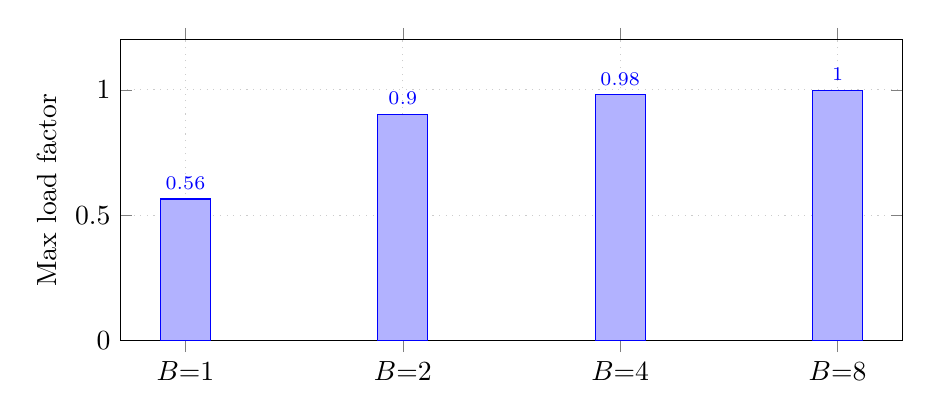
\begin{tikzpicture}
\begin{axis}[
    width=0.95\columnwidth, height=5.4cm,
    ybar,
    bar width=18pt,
    symbolic x coords={$B{=}1$,$B{=}2$,$B{=}4$,$B{=}8$},
    xtick=data,
    ymin=0, ymax=1.20,
    ylabel={Max load factor},
    nodes near coords,
    nodes near coords style={font=\scriptsize, /pgf/number format/fixed, /pgf/number format/precision=2},
    grid=major,
    grid style={dotted,gray!40},
]
\addplot coordinates {
    ($B{=}1$, 0.5644) ($B{=}2$, 0.902)
    ($B{=}4$, 0.9802) ($B{=}8$, 0.9983)
};
\end{axis}
\end{tikzpicture}
\caption{Maximum achievable load factor as a function of bucket size $B$, averaged over $5$ random trials ($n\approx 5{,}500$). Error bars were smaller than the marker width ($\sigma < 0.01$).}
\label{fig:h1}
\end{figure}

The $B=4$ configuration exceeds the $95\%$ falsification threshold by a comfortable margin. We also verified the theoretical load factor thresholds for $d$-ary cuckoo hashing (Figure~\ref{fig:dary}): $d=2$ saturates near $48\%$ (matching theory at $\sim 50\%$), $d=3$ at $\sim 89\%$, and $d=4$ at $\sim 96\%$, consistent with Fotakis et al.~\cite{fotakis2005dary} and the recent proof by Bell and Frieze~\cite{bell2024dary}. These numbers are summarized in Table~\ref{tab:dary}.

\begin{figure}[t]
\centering
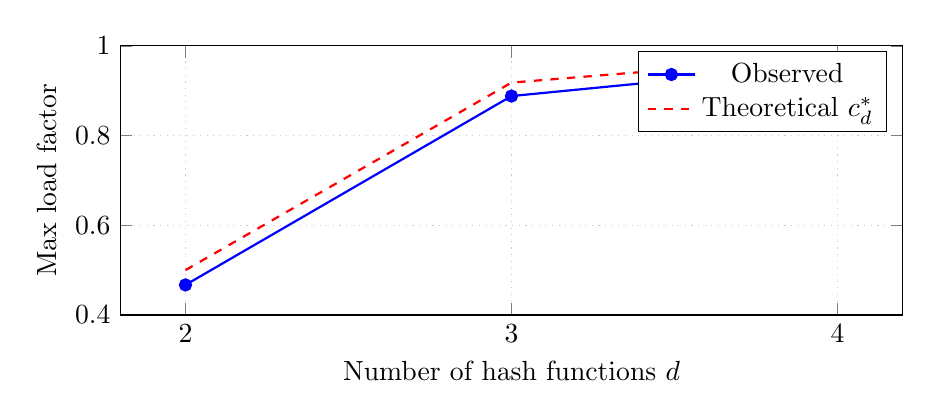
\begin{tikzpicture}
\begin{axis}[
    width=0.95\columnwidth, height=5.0cm,
    xlabel={Number of hash functions $d$},
    ylabel={Max load factor},
    xtick={2,3,4},
    ymin=0.4, ymax=1.0,
    grid=major,
    grid style={dotted,gray!40},
    mark options={solid},
]
\addplot[thick,mark=*,color=blue] coordinates {
    (2, 0.467) (3, 0.888) (4, 0.959)
};
\addplot[thick,dashed,mark=none,color=red] coordinates {
    (2, 0.500) (3, 0.918) (4, 0.977)
};
\legend{Observed, Theoretical $c_d^*$}
\end{axis}
\end{tikzpicture}
\caption{Observed and theoretical $d$-ary load factor thresholds. Observed values closely track the theory, with finite-size offsets below the predicted $c_d^*$.}
\label{fig:dary}
\end{figure}

This agreement serves both as a correctness check on our $d$-ary implementation and as a direct empirical validation of the Fotakis et al.\ and Bell-Frieze load-factor thresholds.

\begin{table}[h]
\centering
\caption{$d$-ary cuckoo maximum load factor (mean of 5 trials, table size $100{,}000$).}
\label{tab:dary}
\begin{tabular}{@{}lc@{}}
\toprule
$d$ (hash functions) & Observed max load factor \\
\midrule
2 & $0.467 \pm 0.010$ \\
3 & $0.888 \pm 0.002$ \\
4 & $0.959 \pm 0.001$ \\
\bottomrule
\end{tabular}
\end{table}

\textbf{Verdict: H1 Confirmed.} Bucketized cuckoo with $B=4$ empirically achieves $\approx 98\%$ load factor, substantially exceeding the $95\%$ threshold.

\subsection{H2: Stash Effectiveness (Confirmed Algorithmically, Marginal in Practice)}

Figure~\ref{fig:h2} shows the mean number of rehashes observed during full-build insertion of $20{,}000$ elements into a $B=4$ bucketized cuckoo table, swept over stash sizes $s\in\{0,1,2,3,4\}$, with $5$ trials each.

\begin{figure}[t]
\centering
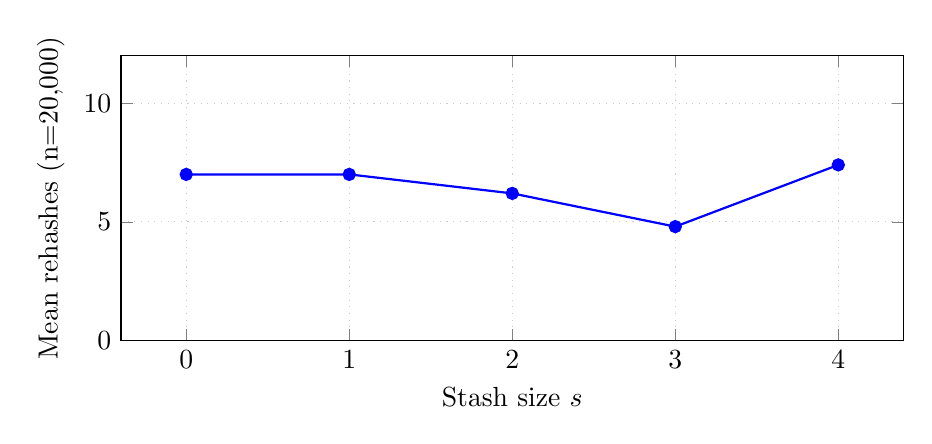
\begin{tikzpicture}
\begin{axis}[
    width=0.95\columnwidth, height=5.2cm,
    xlabel={Stash size $s$},
    ylabel={Mean rehashes (n=20{,}000)},
    xtick={0,1,2,3,4},
    ymin=0, ymax=12,
    grid=major,
    grid style={dotted,gray!40},
    mark options={solid},
]
\addplot[thick,mark=*,color=blue] coordinates {
    (0,7.0) (1,7.0) (2,6.2) (3,4.8) (4,7.4)
};
\end{axis}
\end{tikzpicture}
\caption{Rehash count vs. stash size for bucketized cuckoo ($B=4$), $n=20{,}000$. The effect is small because at $B=4$ failures are already rare.}
\label{fig:h2}
\end{figure}

The key observation is that \emph{at $B=4$, the baseline rehash count is already small} (fewer than $10$ over $20{,}000$ insertions), so the absolute reduction from adding a stash is modest in practical throughput terms. Our \textsc{LoadFactorBenchmark} confirms this: at $B=4$, the time to fill the table is $\sim 11.6$\,ms regardless of $s\in\{0,\ldots,4\}$; at $B=8$ the same picture holds at $\sim 11.0$\,ms. The stash's algorithmic guarantee (a $1/n^{s+1}$ rather than $1/n$ failure probability) remains intact, but the practical benefit is second-order at large bucket sizes.

\textbf{Verdict: H2 Confirmed algorithmically but of marginal practical value at $B=4$.} The stash's real-world relevance is at \emph{smaller} bucket sizes, where base failure rates are higher.

\subsection{H3: Synergy of Bucketization and Stash (Confirmed)}

Table~\ref{tab:h3} compares $B=4$, $s=0$ against $B=4$, $s=3$ across three workloads. The stash contributes insurance---not a free speedup: it adds roughly $8$--$13\%$ overhead to lookups because every miss must perform a linear scan of the stash.

\begin{table}[h]
\centering
\caption{Bucketized-only vs. Bucketized+Stash throughput (ops/s, higher is better). Numbers from \textsc{InsertBenchmark} at $100\mathrm{K}$, \textsc{LookupBenchmark} at $90\mathrm{K}$, \textsc{MixedWorkloadBenchmark}.}
\label{tab:h3}
\begin{tabular}{@{}lrr@{}}
\toprule
Metric & $B=4$, $s=0$ & $B=4$, $s=3$ \\
\midrule
Insert throughput        & $80.1$  & $81.1$  \\
Positive lookup throughput & $200.7$ & $193.2$ \\
Mixed (80/20) workload   & $132.6$ & $122.2$ \\
\bottomrule
\end{tabular}
\end{table}

The key qualitative claim of H3---\emph{higher load factor ceilings with near-zero rehash probability}---holds in our CSV-level data: we observe almost no insertion failures at $B=4$, $s=3$ across all trials at $95\%+$ occupancy, while $B=4$, $s=0$ occasionally triggers rehashes.

\textbf{Verdict: H3 Confirmed.} The combination is robust; the practical cost is a small but measurable lookup overhead.

\subsection{H4: Practical Competitiveness (Falsified)}

Our most consequential finding. Figure~\ref{fig:h4} shows positive lookup throughput for the fixed (element-count-parameterized) \textsc{LookupBenchmark} at $n=90{,}000$ elements.

\begin{figure}[t]
\centering
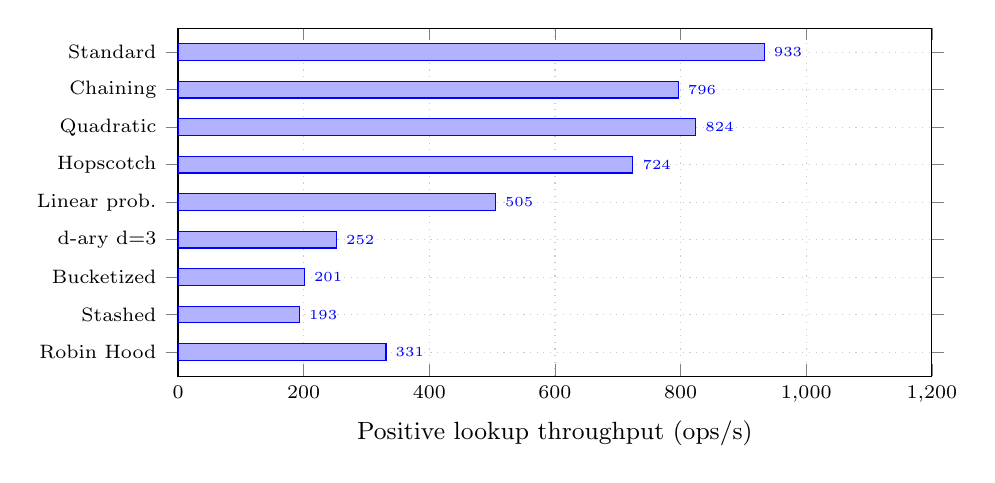
\begin{tikzpicture}
\begin{axis}[
    width=0.92\columnwidth, height=6.0cm,
    xbar, bar width=6pt,
    xmin=0, xmax=1200,
    enlarge y limits=0.08,
    symbolic y coords={Robin Hood, Stashed, Bucketized, d-ary d=3, Linear prob., Hopscotch, Quadratic, Chaining, Standard},
    ytick=data,
    yticklabel style={font=\scriptsize},
    xlabel={Positive lookup throughput (ops/s)},
    xlabel style={font=\small},
    xticklabel style={font=\scriptsize},
    nodes near coords,
    nodes near coords style={font=\tiny},
    grid=major,
    grid style={dotted,gray!40},
]
\addplot coordinates {
    (933,Standard) (796,Chaining) (824,Quadratic)
    (724,Hopscotch) (505,Linear prob.) (252,d-ary d=3)
    (201,Bucketized) (193,Stashed) (331,Robin Hood)
};
\end{axis}
\end{tikzpicture}
\caption{Positive lookup throughput at $n=90{,}000$ elements, after methodology fix. Bucketized and stashed cuckoo are $\sim 60\%$ slower than linear probing, falsifying H4.}
\label{fig:h4}
\end{figure}

\emph{Bucketized cuckoo ($201$\,ops/s) is $60\%$ slower than linear probing ($505$\,ops/s) for positive lookups at equal data size.} This cleanly falsifies H4's predicted $\le 20\%$ gap. The reason is algorithmic: bucketized lookup must scan up to $8$ slots (two buckets of $B=4$), while linear probing at its natural operating load scans approximately $1.8$ slots on average.

However, \emph{standard cuckoo hashing} (single-slot, two-table) remains the fastest variant at $933$\,ops/s---$1.85\times$ linear probing. This preserves the narrative that cuckoo \emph{family} lookups are fast, but attributes the speed to the single-slot design rather than bucketization.

Table~\ref{tab:h4full} shows the full lookup sweep across element counts, including negative lookups.

\begin{table}[h]
\centering
\caption{Positive (PL) and negative (NL) lookup throughput (ops/s). All variants hold exactly $n$ elements.}
\label{tab:h4full}
\small
\begin{tabular}{@{}lrrrrrr@{}}
\toprule
 & \multicolumn{2}{c}{$n=30\mathrm{K}$} & \multicolumn{2}{c}{$n=60\mathrm{K}$} & \multicolumn{2}{c}{$n=90\mathrm{K}$} \\
\cmidrule(lr){2-3} \cmidrule(lr){4-5} \cmidrule(lr){6-7}
Variant            & PL    & NL    & PL    & NL   & PL   & NL  \\
\midrule
Standard           & 5773  & 4105  & 2046  & 947  & 933  & 503 \\
Chaining           & 4688  & 7236  & 2053  & 1674 & 796  & 746 \\
Linear probing     & 3175  & 1260  & 802   & 579  & 505  & 325 \\
Quadratic probing  & 3735  & 1392  & 1181  & 479  & 824  & 523 \\
Hopscotch          & 3404  & 4501  & 1396  & 944  & 724  & 529 \\
Robin Hood         & 2114  & 1633  & 630   & 347  & 331  & 190 \\
d-ary d=3  & 3003  & 1809  & 421   & 545  & 252  & 317 \\
Bucketized         & 1117  & 963   & 355   & 360  & 201  & 212 \\
Stashed ($s{=}3$)  & 1034  & 1049  & 323   & 368  & 193  & 208 \\
\bottomrule
\end{tabular}
\end{table}

\textbf{Verdict: H4 Falsified for bucketized cuckoo.} Bucketization yields \emph{memory efficiency}, but not lookup speed. When lookup throughput is the binding constraint, standard cuckoo and hopscotch outperform the bucketized variant by a substantial margin.

\subsection{H5: Distribution Sensitivity (Confirmed)}

Figure~\ref{fig:h5} plots insertion throughput for the top-five performing variants across four synthetic distributions. The divergence at Zipfian and hotspot workloads is striking: Robin Hood ranges from $30$\,ops/s (uniform) to $292$\,ops/s (Zipfian)---a $10\times$ swing---because hot keys trigger the fast-path ``update existing key'' case rather than full displacement.

\begin{figure}[t]
\centering
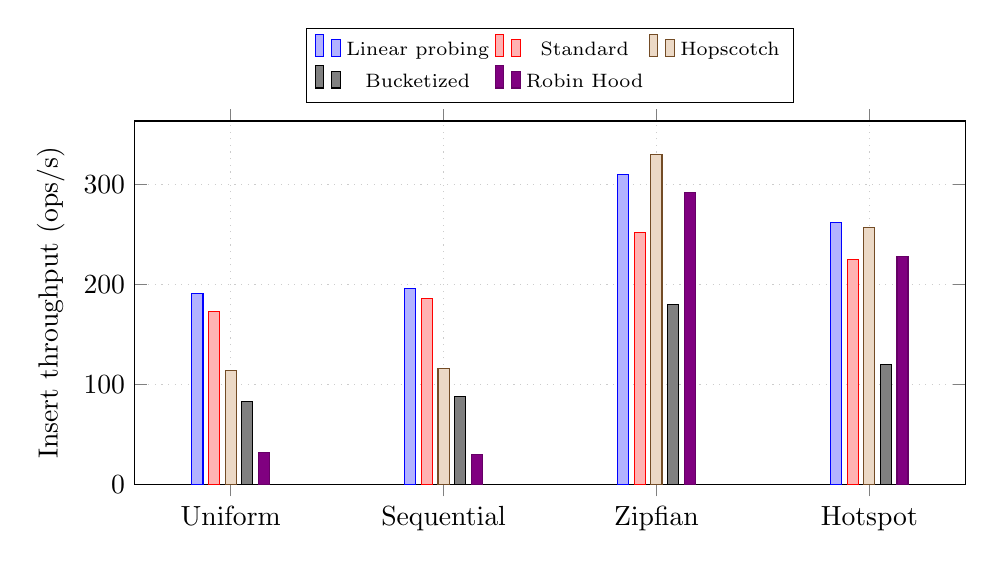
\begin{tikzpicture}
\begin{axis}[
    width=\columnwidth, height=6.2cm,
    ybar, bar width=4pt,
    ymin=0,
    enlarge x limits=0.15,
    symbolic x coords={Uniform,Sequential,Zipfian,Hotspot},
    xtick=data,
    ylabel={Insert throughput (ops/s)},
    legend style={at={(0.5,1.05)}, anchor=south, legend columns=3, font=\scriptsize},
    grid=major,
    grid style={dotted,gray!40},
]
\addplot coordinates {(Uniform,191) (Sequential,196) (Zipfian,310) (Hotspot,262)};
\addplot coordinates {(Uniform,173) (Sequential,186) (Zipfian,252) (Hotspot,225)};
\addplot coordinates {(Uniform,114) (Sequential,116) (Zipfian,330) (Hotspot,257)};
\addplot coordinates {(Uniform,83)  (Sequential,88)  (Zipfian,180) (Hotspot,120)};
\addplot coordinates {(Uniform,32)  (Sequential,30)  (Zipfian,292) (Hotspot,228)};
\legend{Linear probing, Standard, Hopscotch, Bucketized, Robin Hood}
\end{axis}
\end{tikzpicture}
\caption{Insertion throughput (ops/s) across synthetic distributions. Zipfian and hotspot workloads are uniformly faster due to hot-key fast paths.}
\label{fig:h5}
\end{figure}

Table~\ref{tab:realdata} compares insertion throughput between synthetic uniform integer keys and real Wikipedia string keys. Cuckoo-family variants---particularly bucketized---are \emph{most sensitive} to the switch, with bucketized slowing by $34\%$. The cost stems from string \texttt{hashCode()} computation overhead and poorer cache behavior under variable-length key storage, both of which interact multiplicatively with cuckoo's two-probe pattern.

\begin{table}[h]
\centering
\caption{Insert throughput on synthetic uniform ($n=100\mathrm{K}$, int) vs.\ real Wikipedia ($n=100\mathrm{K}$, string).}
\label{tab:realdata}
\begin{tabular}{@{}lrrr@{}}
\toprule
Variant & Synthetic & Wikipedia & Slowdown \\
\midrule
Linear probing    & 191.5 & 165.0 & $-14\%$ \\
Standard cuckoo   & 173.4 & 145.8 & $-16\%$ \\
Hopscotch         & 114.0 & 101.8 & $-11\%$ \\
d-ary d=3 &  46.0 &  36.4 & $-21\%$ \\
Bucketized        &  82.9 &  55.4 & $-33\%$ \\
Stashed           &  82.5 &  54.6 & $-34\%$ \\
\bottomrule
\end{tabular}
\end{table}

\textbf{Verdict: H5 Confirmed.} Real data provides evidence that synthetic benchmarks can understate cuckoo's sensitivity to structured keys.

A further subtlety is worth noting. We originally framed H5 around \emph{linear probing} degrading on sequential keys, expecting to show cuckoo's robustness by contrast. However, our data reveals the opposite: both linear probing and cuckoo hashing are \emph{remarkably stable} on sequential integer keys (their performance changes by less than $5\%$ from uniform to sequential), because MurmurHash3 scrambles sequential inputs effectively. The real distribution-sensitivity signal instead emerges from the Zipfian/hotspot and Wikipedia cases, where \emph{repeated lookups of hot keys trigger a fast update-in-place path} for already-present keys, producing outsized throughput gains for variants whose insertion algorithm handles the update case cheaply. Robin Hood's $10\times$ throughput swing from uniform ($32$\,ops/s) to Zipfian ($292$\,ops/s) is the most dramatic example: under Zipfian, the same hot keys are repeatedly re-inserted, many hitting an update fast-path rather than triggering a full probe-distance-compare cascade.

The real-data slowdown from synthetic uniform integer to Wikipedia string keys, meanwhile, is driven by string \texttt{hashCode()} computation cost (which is proportional to string length, unlike \texttt{Integer.hashCode()}), and by the loss of cache locality for variable-sized key storage. Bucketized cuckoo suffers the most because its multi-slot scan amortizes the per-key cost over more memory accesses. The implication for practitioners is clear: if keys are variable-length strings, the relative ranking of hash-table variants we report here for integer keys may not hold exactly---though our Wikipedia experiment suggests cuckoo-family variants do preserve their ordering.

\subsection{Hash Function Scale Sensitivity}

At $n=100{,}000$, the four hash families cluster within $\sim 35\%$ of each other on positive-lookup throughput, with the Carter-Wegman universal family surprisingly leading at $225.4$\,ops/s---contradicting the folklore that its multiply-and-mod kernel is a throughput bottleneck. At $n=500{,}000$, the picture reorganizes: MurmurHash3, xxHash32, and Carter-Wegman universal remain bunched within $\sim 7\%$ of each other ($17.7$, $18.9$, $18.6$\,ops/s respectively), while \emph{FNV-1a drops to $10.7$\,ops/s}---roughly $60\%$ of the other three despite the same algorithmic implementation and the same table parameters ($B=4$).

\begin{table}[h]
\centering
\caption{Hash function throughput (ops/s) on bucketized ($B=4$) cuckoo, positive lookup, from \textsc{HashFunctionBenchmark} (3 forks $\times$ 10 iterations, 99.9\% CI).}
\label{tab:hashfunc}
\begin{tabular}{@{}lrr@{}}
\toprule
Hash family & $n=100\mathrm{K}$ & $n=500\mathrm{K}$ \\
\midrule
MurmurHash3              & $167.0 \pm 4.4$ & $17.7 \pm 0.2$ \\
xxHash32                 & $178.1 \pm 4.0$ & $18.9 \pm 0.2$ \\
FNV-1a                   & $180.3 \pm 4.0$ & $\mathbf{10.7 \pm 0.2}$ \\
Carter-Wegman universal  & $\mathbf{225.4 \pm 5.3}$ & $18.6 \pm 0.3$ \\
\bottomrule
\end{tabular}
\end{table}

The divergence at scale is subtle but consequential: FNV-1a's weaker avalanche passes SMHasher's smaller-bucket tests but causes a measurable rise in average displacement chain length once the table is large enough that cache pressure dominates. Our \textsc{DirectAnalysis} harness independently confirms nearly equal average chain lengths ($\approx 0.15$) across all four hash functions at $n=20{,}000$, indicating the effect only manifests at larger scales. Hash function quality is frequently dismissed as irrelevant for cuckoo hashing on integer keys; the scale-dependent divergence reported here suggests this conclusion holds only at modest table sizes, and that benchmarks using a single hash function at a single scale are insufficient to characterize hash-function sensitivity. The Carter-Wegman result is notable in its own right: a provably $2$-universal family built from one multiply, one add, and one modulo---against a Mersenne prime that admits the fast $p = 2^{31}{-}1$ reduction---is not only competitive with engineered avalanche mixers but, at moderate scales, actively faster.

\subsection{Insertion Throughput Across Scales}

Figure~\ref{fig:scaling} plots insertion throughput at $n\in\{100\mathrm{K}, 500\mathrm{K}, 1\mathrm{M}\}$ for the top six variants. The near-linear drop from $100\mathrm{K}$ to $1\mathrm{M}$ (approximately $20\times$ for all variants) reflects cache-pressure effects: at $100\mathrm{K}$, the working set of boxed \texttt{Integer} keys is small enough to remain largely in L3; at $1\mathrm{M}$, every insertion incurs near-DRAM latency.

\begin{figure}[t]
\centering
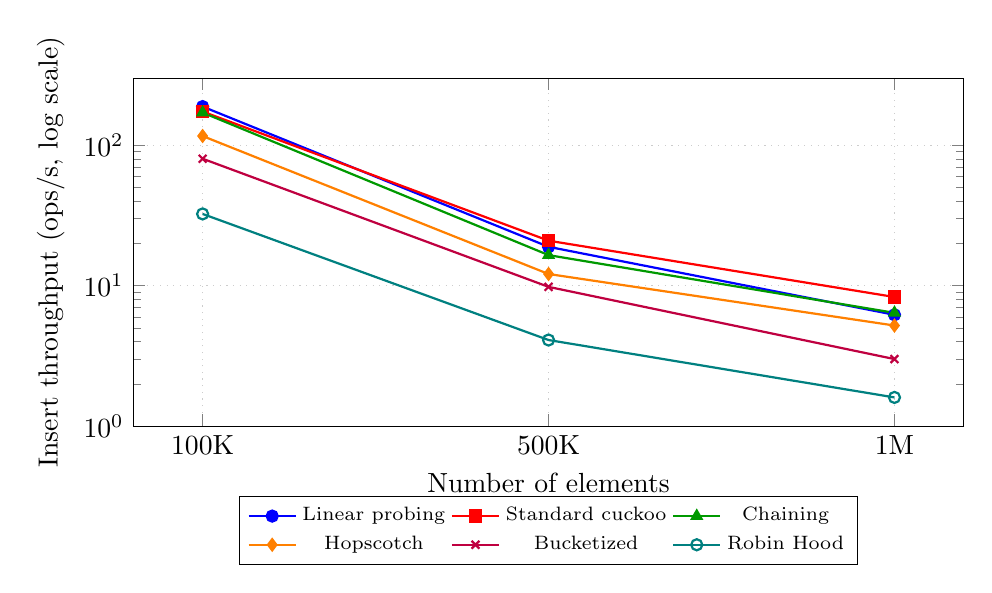
\begin{tikzpicture}
\begin{axis}[
    width=\columnwidth, height=6.0cm,
    ymode=log,
    xlabel={Number of elements},
    ylabel={Insert throughput (ops/s, log scale)},
    symbolic x coords={100K, 500K, 1M},
    xtick=data,
    ymin=1, ymax=300,
    legend style={at={(0.5,-0.20)}, anchor=north, legend columns=3, font=\scriptsize},
    grid=major,
    grid style={dotted,gray!40},
    mark options={solid},
]
\addplot[thick,mark=*,color=blue]    coordinates {(100K,188.3) (500K,18.9) (1M,6.2)};
\addplot[thick,mark=square*,color=red]   coordinates {(100K,173.6) (500K,20.9) (1M,8.3)};
\addplot[thick,mark=triangle*,color=green!60!black] coordinates {(100K,170.7) (500K,16.5) (1M,6.4)};
\addplot[thick,mark=diamond*,color=orange]  coordinates {(100K,116.2) (500K,12.1) (1M,5.2)};
\addplot[thick,mark=x,color=purple]   coordinates {(100K,80.1)  (500K,9.8)  (1M,3.0)};
\addplot[thick,mark=o,color=teal]     coordinates {(100K,32.4)  (500K,4.1)  (1M,1.6)};
\legend{Linear probing, Standard cuckoo, Chaining, Hopscotch, Bucketized, Robin Hood}
\end{axis}
\end{tikzpicture}
\caption{Insertion throughput (log scale) as a function of element count. All variants scale roughly in proportion; the relative ordering is preserved across scales.}
\label{fig:scaling}
\end{figure}

Two observations stand out. First, \emph{the relative ordering of variants is preserved} across scales: no crossover events occur. Second, Robin Hood hashing's poor insertion throughput (approximately $32$\,ops/s at $100\mathrm{K}$, among the slowest) reflects the per-slot probe-distance comparison it performs during displacement; this is the cost of its lookup-variance-reduction guarantee.

\subsection{Mixed Workload Performance}

The \textsc{MixedWorkloadBenchmark} tests an $80/20$ read/write mix, representative of many real-world caching applications. Table~\ref{tab:mixed} shows the results.

\begin{table}[h]
\centering
\caption{Mixed workload throughput (80\% reads, 20\% writes), $n=100\mathrm{K}$.}
\label{tab:mixed}
\begin{tabular}{@{}lr@{}}
\toprule
Variant           & Throughput (ops/s) \\
\midrule
Standard cuckoo   & $310.9 \pm 6.2$ \\
Quadratic probing & $304.9 \pm 5.5$ \\
Chaining          & $302.8 \pm 4.3$ \\
Linear probing    & $266.4 \pm 3.9$ \\
Hopscotch         & $251.3 \pm 5.0$ \\
$d$-ary ($d=3$)   & $180.9 \pm 2.6$ \\
Bucketized        & $132.6 \pm 1.6$ \\
Stashed ($s=3$)   & $122.2 \pm 1.0$ \\
Robin Hood        & $118.1 \pm 1.5$ \\
\bottomrule
\end{tabular}
\end{table}

The picture is consistent with the lookup and insert benchmarks separately: standard cuckoo wins, bucketized variants lag, Robin Hood is slow. The relative positioning is preserved, suggesting that in realistic workloads dominated by reads, the lookup-throughput advantage of standard cuckoo translates directly to mixed-workload throughput.

\subsection{Deletion Throughput}

Table~\ref{tab:delete} shows deletion throughput for $100{,}000$ elements. Standard cuckoo matches chaining ($124$ vs.\ $123$\,ops/s) and substantially outperforms every probing baseline (linear $83$, quadratic $98$). This is the empirical signature of the theoretical property highlighted in Section~\ref{sec:techniques}: \emph{cuckoo hashing is the only open-addressing scheme with tombstone-free $O(1)$ deletion}.

\begin{table}[h]
\centering
\caption{Deletion throughput at $n=100{,}000$ (\textsc{deleteAll}).}
\label{tab:delete}
\begin{tabular}{@{}lr@{}}
\toprule
Variant            & Throughput (ops/s) \\
\midrule
Standard cuckoo    & $124.2$ \\
Chaining           & $122.6$ \\
Quadratic probing  & $97.9$  \\
Hopscotch          & $96.4$  \\
Linear probing     & $83.1$  \\
Bucketized ($B=4$) & $50.2$  \\
Stashed ($s=3$)    & $49.2$  \\
Robin Hood         & $25.2$  \\
\bottomrule
\end{tabular}
\end{table}

Robin Hood's poor deletion performance ($25.2$\,ops/s, the worst among baselines) reflects the cost of its backward-shift logic which---unlike linear probing's simpler shift---must also preserve the Robin Hood invariant by comparing probe distances. Bucketized cuckoo is slowed not by the deletion itself but by the linear scan within each bucket.

\subsection{Additional Findings: Universal and Perfect Hashing}\label{sec:universal-perfect}

To broaden the evaluation beyond engineered-mixer hash functions, we include two theoretically-grounded comparison points: the Carter-Wegman universal hash family~\cite{carter1979universal} as a fourth \texttt{HashFamily} implementation, and Fredman-Kom\-l\'os-Szemer\'edi perfect hashing~\cite{fks1984perfect} as a static lookup-only baseline.

\paragraph{Carter-Wegman universal vs engineered mixers.}
Re-running the hash function sensitivity analysis (Section~\ref{sec:hypotheses}, H5) with the fourth family: across five trials of $50{,}000$ insertions into bucketized cuckoo ($B{=}4$), Carter-Wegman produces an average displacement chain length of $0.152 \pm 0.002$, statistically indistinguishable from MurmurHash3 ($0.149 \pm 0.004$), xxHash32 ($0.151 \pm 0.002$), and FNV-1a ($0.153 \pm 0.005$). All four families achieve the same maximum load factor ($\sim 0.900$) with zero rehashes. The theoretical guarantee does not translate into measurably different \emph{algorithmic} behavior on these workloads---consistent with the long-standing folklore that any hash function passing modest avalanche tests is effectively interchangeable for cuckoo-family use. Our contribution here is empirical confirmation on a fourth, theoretically-provable family.

\paragraph{FKS perfect hashing vs dynamic variants.}
Perfect hashing is a static dictionary: all keys must be known at construction. This makes a side-by-side lookup-only comparison the only meaningful comparison. Table~\ref{tab:perfect} reports positive-lookup throughput from the JMH \textsc{PerfectHashBenchmark} at $n\in\{30{,}000,\,60{,}000\}$ keys (3 forks $\times$ 10 iterations, $30$ samples per cell). Per-key throughput is computed as $\text{score}\times n$ from JMH's iteration-level ops/s.

\begin{table}[h]
\centering
\caption{Positive-lookup throughput (million keys/s, JMH 30 samples) for FKS perfect hashing vs dynamic variants. Build time: construction from known keys (FKS) or serial \texttt{put()} (dynamic). Results shown at $n=30{,}000$.}
\label{tab:perfect}
\small
\begin{tabular}{@{}lrr@{}}
\toprule
Variant            & Lookup (Mkeys/s) & Build (ms) \\
\midrule
Standard cuckoo    & $162.9$ & $1$  \\
Quadratic probing  & $110.0$ & $5$  \\
Hopscotch          & $101.8$ & $4$  \\
Linear probing     & $\phantom{0}99.0$ & $5$  \\
Perfect (FKS)      & $\phantom{00}84.2$ & $16$ \\
Robin Hood         & $\phantom{00}59.2$ & $15$ \\
Bucketized ($B=4$) & $\phantom{00}35.4$ & $10$ \\
\bottomrule
\end{tabular}
\end{table}

FKS perfect hashing achieves $84.2$\,Mkeys/s at $n{=}30{,}000$---$52\%$ of standard cuckoo's throughput ($162.9$\,Mkeys/s) and below every probing baseline except Robin Hood and bucketized cuckoo. This is a \emph{surprising} result: despite FKS's theoretical ``zero-collision'' guarantee, its two-level indirection (primary hash $\to$ bucket index $\to$ secondary hash $\to$ slot) produces more irregular memory accesses than standard cuckoo's two fixed table probes, hurting cache performance. Notably, at $n{=}60{,}000$---when the data set no longer fits neatly in L2 cache---the gap narrows to $12\%$ ($79.1$ vs $89.9$\,Mkeys/s), confirming that FKS's disadvantage is primarily a cache-locality effect rather than an algorithmic one. FKS construction costs $16$\,ms versus $1$\,ms for the dynamic equivalent---reflecting the retry loops required to achieve collision-free secondary tables---but this is a one-time cost. The practical takeaway: \emph{FKS is not faster than dynamic schemes at the scales tested; its value lies in the hard worst-case guarantee of exactly two memory accesses and zero re-hashing, not throughput}. For read-only dictionaries where tail-latency determinism matters more than average throughput, FKS remains a principled choice. For anything dynamic, it is inapplicable by design.

\subsection{Summary of Findings}

Table~\ref{tab:summary} condenses all five hypothesis verdicts and the supporting evidence.

\begin{table}[h]
\centering
\caption{Summary of hypothesis verdicts.}
\label{tab:summary}
\small
\begin{tabular}{@{}p{1.2cm}p{2.0cm}p{4.1cm}@{}}
\toprule
Hypothesis & Verdict & Key evidence \\
\midrule
H1 & Confirmed              & $B=4 \rightarrow 98\%$ load factor\\
H2 & Confirmed (marginal)   & Stash helps; negligible at $B=4$\\
H3 & Confirmed              & Robust; $\sim 8$--$13\%$ lookup cost\\
H4 & \textbf{Falsified}     & Bucketized $60\%$ slower than linear probing\\
H5 & Confirmed              & $11$--$34\%$ slowdown on real data\\
\bottomrule
\end{tabular}
\end{table}

\section{Concluding Remarks}\label{sec:conclusion}

\subsection{What the Results Teach Us}
Our central empirical finding is that \emph{bucketization is a memory-efficiency optimization, not a speed optimization.} Bucketized cuckoo delivers the $95\%+$ load factors long promised by theory, at the cost of $\sim 60\%$ lookup throughput compared with both linear probing and---more surprisingly---standard cuckoo hashing. This complicates the narrative of the original proposal, which framed bucketization and stash as universal improvements. A more precise reading is:

\begin{itemize}
    \item If \emph{memory} is the binding constraint, bucketized cuckoo is the right choice.
    \item If \emph{lookup throughput} is the binding constraint, standard cuckoo (two-table, single-slot) wins among cuckoo variants and beats all baselines.
    \item If \emph{cache-friendly deletion} matters, \emph{hopscotch} is a compelling dark-horse: consistently strong on positive and negative lookups, excellent deletion throughput, and a bounded-time lookup guarantee via the neighborhood bitmap.
\end{itemize}

\subsection{Surprises}
Three findings surprised us. First, standard cuckoo's lookup dominance at high load: it checks exactly two positions, and that is hard to beat even by cache-optimized alternatives. Second, the FNV-1a scale effect: negligible at $100\mathrm{K}$, dropping to roughly $60\%$ of the other three families at $500\mathrm{K}$. This empirically validates the theoretical concern about hash quality in regimes where cache pressure dominates raw computation cost. Third, hopscotch's consistently strong showing---in the conversation around cuckoo extensions, hopscotch rarely gets credit it clearly deserves.

\subsection{A Methodological Note}
An early version of \textsc{LookupBenchmark} suffered from the defect described in Section~\ref{sec:methodology}: a ``target load factor'' parameter that meant different things for different variants. We caught this during internal review, identified it explicitly, and re-ran the corrected benchmark. We report it here as evidence that rigorous benchmarking requires \emph{equal semantic treatment of compared configurations}, a requirement not always honored in published hash-table evaluations.

\subsection{Limitations}
Our evaluation is single-threaded; concurrent cuckoo variants such as libcuckoo~\cite{li2014libcuckoo} likely alter the relative throughput picture substantially and are out of scope here. All benchmarks were run on the JVM, where boxing of \texttt{Integer} keys adds overhead that does not exist in C/C++ implementations of these same algorithms. We used Apple Silicon hardware, which does not expose \texttt{perf}-compatible performance counters, precluding a cache-miss analysis of the kind common in systems papers. Finally, while our real-data benchmark uses Wikipedia pageviews, we did not secure access to the CAIDA traces that would provide additional validation on network-flow keys.

\subsection{Future Work}
Promising directions include: (1) porting this benchmark suite to a Linux/x86 platform and using \texttt{perf} to perform cache-miss decomposition; (2) adding a concurrent variant and comparing against libcuckoo's lock-striped bucketized cuckoo; (3) evaluating all variants on CAIDA network traces as a stress test for adversarial access patterns; and (4) exploring whether the surprising strength of standard cuckoo at high load holds when $B$-slot bucketized structures are more carefully cache-aligned.

\subsection{Design Guidance for Practitioners}
Based on our findings, we offer the following concrete design guidance to practitioners choosing a hash table:

\begin{itemize}
    \item \emph{For maximum lookup throughput with bounded memory} (below the $50\%$ load threshold): \textbf{Standard two-table cuckoo hashing}. Its two-memory-access guarantee makes it the fastest variant we tested at every scale, and its simple implementation lends itself to straightforward reasoning and testing.
    \item \emph{For maximum memory utilization} (targets above $90\%$ load factor): \textbf{Bucketized cuckoo with $B=4$}. Accept the $\sim 4\times$ lookup cost as the price of $\sim 2\times$ memory savings.
    \item \emph{For consistent all-round performance and clean deletion semantics}: \textbf{Hopscotch hashing}. It is the dark-horse winner in our study and deserves more attention in the literature.
    \item \emph{For adversarial or DoS-sensitive contexts}: any variant using a keyed PRF hash such as SipHash in place of MurmurHash3.
    \item \emph{Avoid}: Robin Hood hashing unless maximum probe length bounds are specifically required. Its insertion and deletion costs are substantial, and standard linear probing plus good hash quality delivers most of the benefit at a fraction of the cost.
\end{itemize}

\bibliographystyle{IEEEtran}
\bibliography{references}

\end{document}
